\chapter{Pair Interaction LGCA}
Pair-interaction automata (PI) constitute another branch that successfully evolved from HPP model, somewhat in contrast to FHP.
To put it in a nutshell, FHP changed the rectangular grid for hexagonal, and thus obtained better rotational symmetry, increased the degree of freedom of the nodes and added new collision states. 

The pair-interaction model preserves the HPP rectangular lattice, but the degrees of freedom in the node are incremented by the artificial definition of momentum.
%In FHP and HPP, momentum of the particle corresponds to its lattice velocity, or equivalently, to the cell that the particle occupies.
Momenta has no longer same direction as the lattice velocities, but they constitute an inner degree of freedom of the particle, that might change in the collision, independently of the lattice velocity.
Although the differentiation in momentum and velocity might seem odd at the first glance, we will show that it leads to the physically correct microdynamics and offers us very efficient algorithm for implementation.

\bigskip
We will explore theory of Pair Interaction automaton in arbitrary dimension later on, but to get good understanding of the pair-interactions, we start with its $2$D version, so we can explain the theory graphically.

\section{User-friendly guide to Pair interactions}

\subsection{Pair-interactions automaton in two dimensions}

Geometry of the lattice is same as for HPP model. It consists of nodes arranged in the rectangular grid:

\begin{figure}[htbp]
 \centering 
 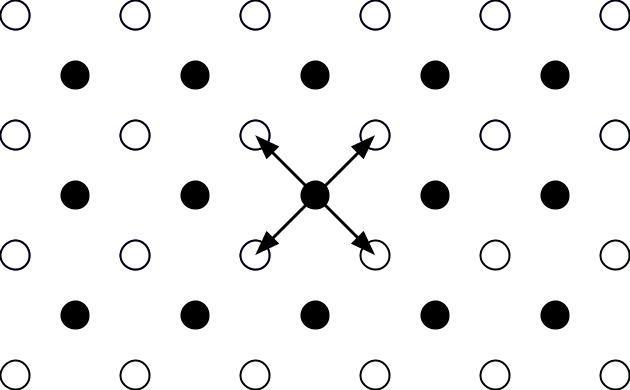
\includegraphics[width=0.9\textwidth]{./img/pi_grid}
 \label{2dgrid}
 \caption{Lattice of 2D Pair Interaction automaton}
\end{figure}

%Every node (the cirlce on the picture above) is connected to 4 diagonal neighbors.
Let us consider that in the time-step $t$ only the black nodes are occupied (e.g. with odd Cartesian idices). Then in the next step $t+1$, only the white nodes (with even indices) are occupied. 
So the set of occupied points alternate with every time step, which offers very efficient implementation, because we can perform propagation on the single data-structure.

\bigskip

\subsection{Node in detail}

Let us look at the node in a more detail
%If we look on the node in more detail, it looks like this:
\begin{figure}[H]
 \centering 
 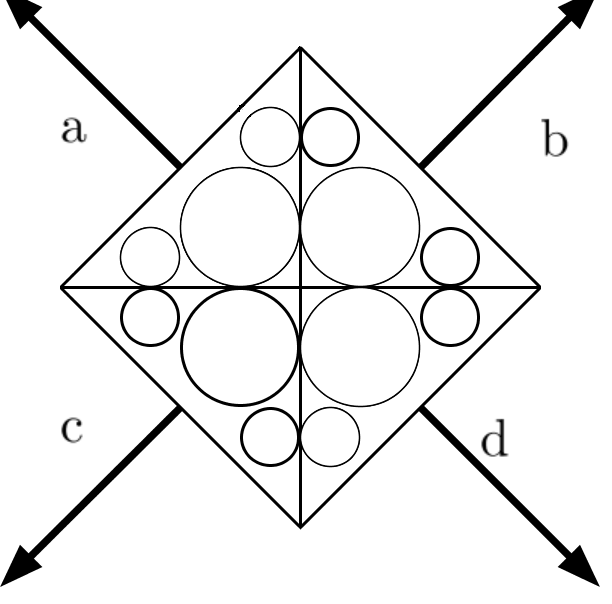
\includegraphics[width=0.5\textwidth]{./img/node_empty}
 \label{empty}
 \caption{An empty node}
\end{figure}

\newpage
It consists of 4 cells ( \textbf{a,b,c,d} ) that are represented by 3 bits:
% on the picture. Each cell is represented by 3 bits:
one mass bit (a big circle) and two momentum bits (small circles).

The node on the picture above is empty (all bits are set to zero).

Here we have another example of a node:
\begin{figure}[htbp]
 \centering 
 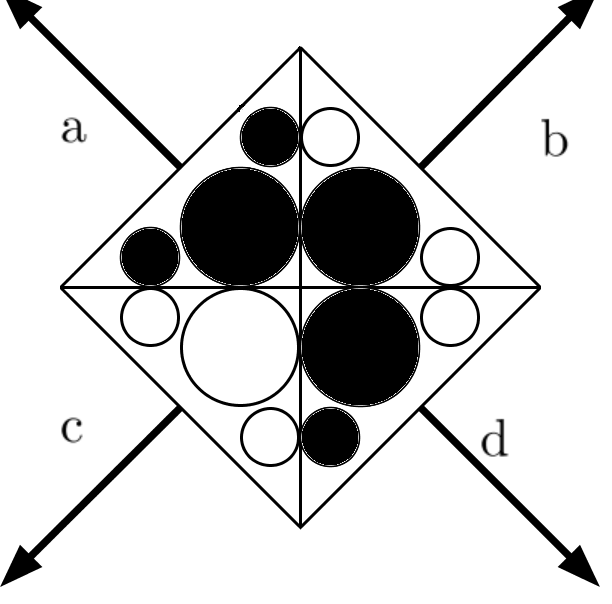
\includegraphics[width=0.5\textwidth]{./img/node_1}
 \label{pre_collision}
 \caption{State of a node before collision}
\end{figure}

In this node, there are particles in the cells a,b,d (mass bit is set to 1 - the big circle is black).

Particle in the cell \textbf{a} is standing (both momentum bits are 0).

Particle in the cell \textbf{b} has momentum in direction [1,1] and particle in the cell \textbf{d} has momentum in direction [0,1].

\subsection{Update rules}
Following rules are true of every lattice-gas cellular automaton.

\begin{enumerate}
\item Lattice is changing in discrete time steps
\item Update rules are \textbf{local}. It means that state of the cell in the next step is determined by the current state of the cell itself and its four neighbors. Hence we can resolve update of the lattice node by node, which can be carry out parallely.
\item If this cellular automaton really simulates fluid dynamics and is physically realistic, update rule needs to conserve \textbf{mass, momentum and angular momentum}.
\end{enumerate}

Update of the lattice is accomplished in two distinct steps -- collision and propagation.

\subsection{Collision}
Collision changes configuration of the single nodes respecting two constraints -- number of particles and total momentum in the node is conserved. In this model, it is performed by the pair-interaction algorithm:
\begin{enumerate}

\item The cells are paired in X direction:
\begin{figure}[H]
 \centering 
 \includegraphics[width=0.3\textwidth]{../obrazky/x-interaction}
 \label{xinter}
 \caption{Pairs in X-direction}
\end{figure}

\item Then we swap the bits in the pairs so that total momentum in the pair is preserved. Therefore, node in \ref{pre_collision} changes to

\begin{figure}[H]
 \centering 
 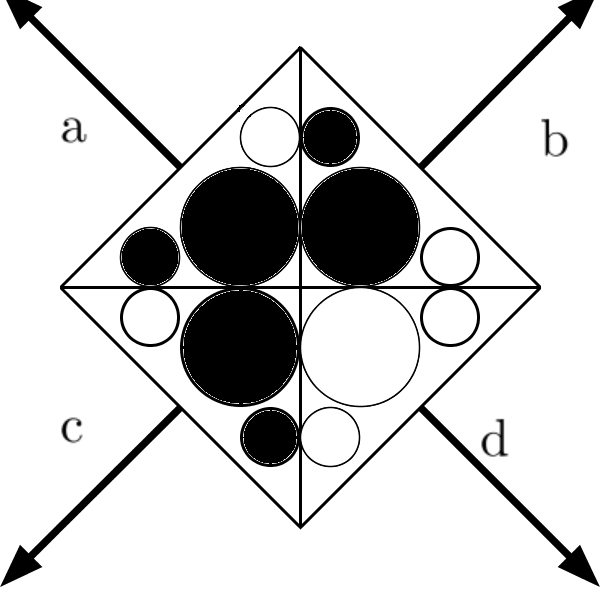
\includegraphics[width=0.5\textwidth]{./img/node_2}
 \label{colision1}
 \caption{State of the node after pair-interaction in X direction}
\end{figure}

\item Then, the cells are paired in Y direction
\begin{figure}[htbp]
 \centering 
 \includegraphics[width=0.3\textwidth]{../obrazky/y-interaction}
 \label{yinter}
 \caption{Pairs in Y-direction}
\end{figure}

\item we change the configuration in these pairs preserving mass and momentum in the node. Hence, the node in \ref{colision1} changes into:
 \begin{figure}[htbp]
 \centering 
 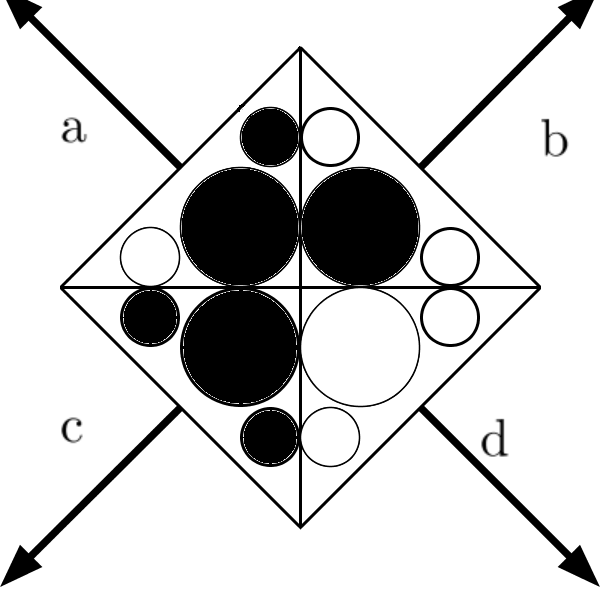
\includegraphics[width=0.5\textwidth]{./img/node_3}
 \label{colision2}
 \caption{State of the node after pair-interaction in Y-direction}
\end{figure}
\newpage
\end{enumerate}

In total, there is only 17 possible configurations of the pairs, so the pair-interaction can be resolved by This table is same for Pair-interaction automata of any dimension, which is the great advantage comparing to other methods.
\newpage
\begin{figure}[htbp]
 \centering 
 \includegraphics[width=0.7\textwidth]{../obrazky/transitions}
 \label{transitions}
 \caption{All admissible pair-interactions}
\end{figure}

\section{Propagation:}
Same as for HPP, particles propagates from a node along $4$ lattice vectors to the neighboring nodes. Of course, all the bits from the cell propagates with the particle (the mass and momentum bits alike)


\section{Pair-interaction cellular automaton in 3D and arbitrary dimension}
\begin{center}
    \begin{tabular}{| l | l | l | l |}
    \hline
    \multicolumn{3}{|c|}{DIFFERENCES BETWEEN \textbf{2}D AND \textbf{N}D PAIR INTERACTION}\\ \hline
     & \textbf{2dim PI CA} & \textbf{Ndim PI CA} \\ \hline
    \textbf{nodes} & $4$ cells arranged into square & $2^D$ cells arranged in hypercube \\ \hline
    \textbf{cells} & 1 mass bit, 2 momentum bits  & 1 mass bit, N momentum bits \\ \hline
    \textbf{neighbors} & node has 4 neighbors & node has $2^D$ neighbors  \\ \hline
    \end{tabular}
\end{center}

Generalization of this automaton to the arbitrary dimension D is very straight-forward. Instead of formalism that Nasilowski used in his founding article \cite{nasilowski}, we will use formalism that we already established for FHP model.

State of the node will be denoted by $\bm{n}(t,\bm{r})$, where $\bm{r}$ is its position on the lattice and $t$ is the current time step. $\bm{n}(t,.)$ represents the whole lattice at time $t$. When possible, we will skip the time variable and use only $\bm{n}(.)$.

Each node consists of $2^D$ cells
\begin{equation}
\bm{n} = (n_1, n_2, ... , n_{2^D})
\end{equation}
or $2^D(D+1)$ bits
\begin{equation}
\bm{n} = \big\{ n_{i\alpha} \in \big\{0,1\big\},~i = 1..2^D, ~\alpha = 0,1,...D\big\}
\end{equation}
where $i$ is index of the cell, index $\alpha = 0$ stands for the mass bit, and $\alpha = 1,2,..D$ stands for the momenta bits of the cell.

\section{Update}
The evolution of the lattice happens in discrete time steps $\mathcal{U}$
\begin{equation}
\mathcal{U} \bm{n}(t,.) = \bm{n}(t+1,.)
\end{equation} 
Update operator $\mathcal{U}$ is the composition of two operators, collision $\mathcal{C}$ and propagation $\mathcal{P}$
\begin{equation}
\mathcal{U} = \mathcal{P} \circ \mathcal{C}.
\end{equation} 

\section{Collision}

The purpose of collision is to change the state of the node $\bm{n}$ into new state $\bm{n'}$ such that 2 conditions are fulfilled:

\begin{enumerate}
\item \textbf{Collision operator is one-to-one}

If $\mathcal{C}: \bm{n} \rightarrow \bm{n'}$,
then $\mathcal{C}: \bm{n'} \rightarrow \bm{n}$.

This reversibility condition allows us to apply Gibbs formalism later on.

\item \textbf{Collision preserves mass and momentum in the nodes}

Mass and momentum are given by
\begin{equation}
m_0 = \sum_i n_{i0}
\end{equation}
\begin{equation}
p_j = \sum_i c_{ij} n_{ij},~j=1,2,...D
\end{equation}
Using these definitions, conservation of mass and momentum can be expressed by
\begin{align}\label{mmc}
\begin{split} 
m_o = m'_o &~~ \Leftrightarrow ~~ \sum_i n_{i0} = \sum_i n'_{i0}, \\
p_j = p'_j &~~ \Leftrightarrow ~~ \sum_i c_{ij} n_{ij} = \sum_i c_{ij} n'_{ij}, ~j=1,2,... D 
\end{split}
\end{align}
\end{enumerate}
The simplest collision rule fulfilling these conditions would be identity
\begin{equation}
\mathcal{I}:\bm{n} \rightarrow \bm{n}
\end{equation}
but this "non-collision" would lead to undesired, non-physical invariants.
On the contrary, we want to change as many bits in the node as possible, to reduce the mean free path of the particles. Physically, it minimizes the shear viscosity and allow us to reach higher Reynolds numbers in the simulations.

\subsection{Collision algorithm}
Collision rule that fulfills all the requirements above turned out to be really simple. It was explained graphically in the previous section, now we state it more formally for an arbitrary dimension D.
The algorithm consists of D steps.
In each step ($d=1...D$), we create pairs of the cells in $d^{th}$ direction, such that $c_{id} = -c_{jd}$ and $c_{i\alpha} = c_{j\alpha}$ for $\alpha \neq d$.
If $n_{id} = n_{jd}$ (it means that in direction $d$, momentum of the pair is zero), we swap the states of the cells $n_i$ and $n_j$ without changing the total momentum of the pairs.
Because all the pair-interactions conserved the momentum, the total momentum in the node is conserved by the collision.

\section{Equilibrium statistics}
We start by revoking the basic equation of the microdynamics
\begin{equation} \label{over2}
\bm{n}(t+2,.) = \mathcal{U}^2 \bm{n}(t,.)
\end{equation}
We remind that $n(.)$ represents the whole lattice, while $n(\bm{r})$ represents the state of the node at $\bm{r}$.

As we already mentioned, the occupied parts on the lattice alternate every time-step, so we can compare only states over the two time steps.

The microdynamical equation \ref{over2} implies conservation of probabilities
\begin{equation} \label{cp}
P(t,\bm{n}(.)) = P(t+2,\mathcal{U}^2\bm{n}(.))
\end{equation}
where $P(t,n(.))$ is the probability that lattice is found in the state $n(.)$ from the statistical ensable of automata.

\subsection{Gibbs distribution}

Before we proceed, it is handy to define the \textbf{hypermomentum} $m_{\alpha}$, where $m_{0}$ is the mass, and $(m_1,m_2,...,m_D)$ is the momentum. 

From now on, the Greek index $\alpha$ will run trough the $\{0,1,2,...,D\}$ and will signalize that hypermomentum is used, while Latin $j$ runs over $\{1,2,...D\}$ and signalizes the standard momentum.

The Gibbs distribution is defined for this model as
\begin{equation}
P^E(n(.)) = \frac{W(n(.))}{Z}
\end{equation}
where
\begin{equation}
W(n(.)) = \exp(-\sum_{\alpha = 0}^D \mu_{\alpha} m_{\alpha}(.)),
\end{equation} 
$Z$ is the partition function
\begin{equation}
Z = \sum_{n(.))} W(n(.)).
\end{equation}
and the $\mu_{\alpha}$ are the intensive parameters conjugated to the hypermomentum $m_{\alpha}$. 

Let us inspect if the Gibbs distribution fulfills the conservation of probabilities required by \ref{cp}.

The total momentum of the whole lattice $\mathcal{L}$ is given by
\begin{equation} \label{momentum}
m_{\alpha}(.) = \sum_{\bm{r} \in \mathcal{L}} c_{i\alpha} n_{i\alpha}(\bm{r}),~\alpha=0,1,..D.
\end{equation}

Conservation of local momenta \ref{mmc} implies conservation of the total momentum
\begin{equation}
m_{\alpha}(.) = m'_{\alpha}(.),~\alpha=0,1,..D
\end{equation}
that immediately implies conservation of the Gibbs probability
\begin{equation}
P^E(t+2,\mathcal{E}^2n(.)) = P^E(t,n(.)).
\end{equation}.
So the $P^E(t,(n.))$ is the stationary solution of \ref{cp}, which means it is the equilibrium distribution for our model. However, the Gibbs distribution represents only one class of the stationary solutions. If there were additional extensive dynamical invariants independent of momenta and mass (e.g. Zanetti's invariants for FHP and FCHC bmodel), there would arise conjugated intensive parameters, corresponding to other equilibrium distributions. However, due to the alternating lattice, this model is free of Zanetti's invariants.

\bigskip

The additivity of the momentum cell by cell on the lattice (equation \ref{momentum}) implies
\begin{equation}
P^E(n(.)) = \prod_{i,\bm{r} \in \mathcal{L}} P^E(n_i(\bm{r}))
\end{equation}
which means that there is no statistical correlation between the cells.
Again,
\begin{equation}
P^E(n_i(\bm{r})) = \frac{W(n_i(\bm{r}))}{Z},
\end{equation}
with
\begin{equation} \label{mprobab}
W(n_i(\bm{r}))=exp(-\sum_{\alpha = 0}^D\mu_{\alpha}c_{i\alpha}n_{i\alpha}(\bm{r})) = \prod_{\alpha=0}^Dexp(-\mu_{\alpha}c_{i\alpha}n_{i\alpha}(\bm{r})) = \prod_{\alpha = 0}^D W(n_{i\alpha}(\bm{r}))
\end{equation}
and
\begin{align*}
Z_i = \sum_{n_i} W(n_i(\bm{r})).
\end{align*}
The probability that the cell is occupied by a particle is
%Let us denote the probability that the cell is occupied by
\begin{align*}
\rho_i \equiv \langle n_{i0} \rangle = \frac{1}{Z_i}
\end{align*}
and the probability that the particle has non-zero $i^{th}$ component of the momentum
\begin{align*}
\sigma_{ij} \equiv \langle n_{ij} | n_{i0} = 1 \rangle = \frac{W(n_{ij}}{Z_i}.
\end{align*}
Rather technical solution of the two equations above shown in the Appendix B of \cite{nasilowski} leads to
\begin{equation} \label{form1}
\rho_i := f\big(\mu_0 + \sum_{j=1}^d ln f(-\mu_j v_j) \big), \quad \sigma_{ij} = f(\mu_j v_j),
\end{equation}
where
\begin{align*}
f(\lambda) := \frac{1}{1 + e^{\lambda}}.
\end{align*}

Because the lattice vectors are normalized and the single node contains $2^D$ lattice vectors, the volume of the node is
\begin{align*}
V = 2^D.
\end{align*}
Finally, we can define the mass density
\begin{equation}
\rho = 2^{-D} \sum_i \rho_i
\end{equation}
and the momentum density
\begin{equation}
q_j := 2^{-D} \sum_i c_{ij} \langle n_{ij} \rangle = 2^{-D} \sum_i c_{ij} \rho_i \sigma_{ij}, \quad j=1,2...D.
\end{equation}
In the next section, we will also use \textbf{hypermomentum} density
\begin{equation} \label{hypermom}
q_{\alpha} := 2^{-D} \sum_i c_{i\alpha} \langle n_{i\alpha} \rangle,~\alpha = 0,1,2...D,
\end{equation}
where $q_0$ is the mass density $\rho$, and $(q_1,q_2,...q_D)$ is the momentum density.

We can use the above definitions to solve equations \ref{form1} in terms of $\rho$ and $\bm{q}$. To find the solution in the closed-form is not possible, but one can find the asymptotic solution for small $\bm{q}$, derived in the Appendix B of \cite{nasilowski}.
\begin{align} \label{hypequi}
\begin{split}
\rho_i &= \rho + 2 \frac{1-\rho}{2-\rho} \bm{v}.\bm{q} + 2 \, \frac{(1-\rho)(1-2\rho}{(2-\rho)^2 \rho} \, \big[(\bm{v}.\bm{q})^2 - q^2 \big] + O(q^3), \\
\sigma_{ij} &= \frac{1}{2} + \frac{v_j q_j}{(2-\rho)\rho} + O(q^3).
\end{split}
\end{align}

\section{Hydrodynamic description}
The quantities of our interest are the so-called \textit{collisional invariant}. These quantities do not change by the collisions, but vary slowly in time and space.
On the most general level, they are temperature, mass and momentum, and the system they describe is in local equilibrium. 

In this section, the system is assumed to be near its local equilibrium, so in the first approximation, it can be described as the local equilibrium state given by \ref{hypequi} with the hypermomentum as its only parameter:
\begin{align*}
\begin{split}
\rho_i^0 = \rho_i^0(q_{\alpha}), \\
\sigma_{i\alpha}^0 = \sigma_{i\alpha}^0(q_{\alpha}),
\end{split}
\end{align*}
% As we already mentioned, this assumption is natural, as the fluid relaxes to its local equilibrium in matter of $10^{-13}$ seconds.

We are looking for the hydrodynamic equations of the form
\begin{align} \label{hydroeq}
\frac{\pd q_{\alpha}}{\pd t} = - \sum_k \nabla_k Q_{\alpha k},
\end{align}
where the $Q_{\alpha k}$ is the hypermomentum flux tensor. The first approximation of this equation
\begin{align*}
\frac{\pd q_{\alpha}}{\pd t} = - \sum_k \nabla_k Q^0_{\alpha k}(q_{\alpha})
\end{align*}
is time-reversal and symmetric, so it cannot capture the viscosity and other friction effects.
 
In order to proceed, we need to expand the functionals $ p_{i\alpha} := (\rho_i,\sigma_{ij})$ and $Q_{\alpha k}$ in the Chapman-Enskog series
\begin{align} \label{distrib}
p_{i \alpha} = p_{i \alpha}^0(\bm{q}) + \sum_{\beta j} R_{i \alpha \beta j}(\bm{q}) \nabla_{j} q_{\beta} + O(\nabla^2),
\end{align}
\begin{align} \label{momentflux}
Q_{\alpha k} = Q_{\alpha k}^0(\bm{q}) - \sum_{\beta j} T_{\alpha \beta k j}(\bm{q}) \nabla_{j} q_{\beta} + O(\nabla^2),
\end{align}
where the tensor $T_{\alpha \beta k j}$ plays the role of the diffusion coefficients.
Note that this expansion is justified only for sufficiently small lattice spacing $\Delta x$, because
\begin{align*}
O(\nabla^k) = O((\Delta x)^{-k}).
\end{align*}

The unknown terms in the equations \ref{distrib} and \ref{momentflux} must be consistent with the microdynamics of our model, and that is the recipe to calculate them.
The details of this calculation are shown in Appendix A of \cite{nasilowski}, we will just summarize the main results.

The momentum flux tensor in the first approximation reads
\begin{align} \label{mft1ap}
\begin{split}
g^0_k := Q^0_{0k} &= 2 \frac{1 - \rho}{2 - \rho} q_k + O(\bm{q}^3), \\
Q^0_{jk} &= \Big( \frac{\rho}{2} - 2 \frac{(1-\rho)(1-2\rho)}{(2-\rho)^2\rho} q_j^2 \Big) \delta_{jk} + 4 \frac{(1-\rho)^2}{(2-\rho)^2} q_j q_k + O(\bm{q}^3).
\end{split}
\end{align}
We have split the hypermomentum flux tensor into its mass component $\bm{g}$ and the ordinary momentum tensor $Q_{jk}$ to obtain the hydrodynamic equations in the familiar form.

\section{Euler equations}
If we substitute these $\bm{g}^0$ and $Q_{jk}^0$ into the hydrodynamic equations \ref{hydroeq}, we obtain
\begin{align}
\begin{split} \label{O2}
\pd_t \rho + \bm{\nabla.} \Big[ \Big( \frac{10}{9} - \frac{8}{9} \Big) \bm{q} \Big] &= 0,\\
\pd_t q_j + \sum_k \nabla_k \Big[\frac{\rho}{2} \delta_{jk} + \frac{8}{9}q_j\,q_k \Big] &= 0,
\end{split}
\end{align}
that are analogous to the compressible Euler equations
\begin{align}
\begin{split}
\pd_t \rho + \bm{\nabla . q} = 0, \\
\pd_t q_j + \sum_k \nabla_k \big[ p(\rho) \, \delta_{jk} + \frac{1}{\rho} \, q_j \, q_k \big]= 0.
\end{split}
\end{align}

%The underlaying reason why this anisotropic term appears is the absence of Galilei invariance in the automaton.

Unfortunately, the tensor $Q_{jk}^0$ from \ref{mft1ap} possesses non-physical anisotropy, due to the term proportional to $q^2_j \delta_{jk}$, and thus the automaton's hydrodynamics is not equivalent to that of physical fluid.

Notice, however, that if we set density to be constant $\rho = 1/2$, the anisotropic term vanishes and we obtain the incompressible inviscid equations
\begin{align}
\begin{split}
\bm{\nabla . q} &= 0, \\ 
(\pd_t + \frac{8}{9}\bm{q.\nabla})\bm{q} + \frac{1}{2} \bm{\nabla} \rho &= 0.
\end{split}
\end{align}
Comparing them to the physical incompressible Euler equations
\begin{align} \label{ideal_phys}
\begin{split}
\bm{\nabla . u} &= 0, \\
(\pd_t + \bm{u.\nabla})\bm{u} + \nabla \Phi &= 0,
\end{split}
\end{align}
we can easily see that they are equivalent and can be transformed into each other by
\begin{align} \label{transformers}
\Phi = \frac{4}{9} \rho, \quad \bm{u} = \frac{8}{9} \bm{q}.
\end{align}
So our model perfectly simulates the ideal fluid (obeying incompressible Euler equations) with the kinematic pressure $\Phi$ and the hydrodynamic velocity $\bm{u}$ defined by \ref{transformers}.
This hydrodynamic velocity can be interpreted as the momentum convection velocity, which differs from the mean velocity $\bm{w}$ of the particles
\begin{align}
\bm{w} = \frac{\langle \sum_i v_i n_{i0} \rangle}{\langle \sum_i n_{i0} \rangle} \approx \frac{2(1-\rho)}{(2 - \rho) \rho}\bm{q}.
\end{align}
%and for $\rho = 1/2$ we have
%\begin{align*}
%\bm{w} = \frac{3}{2} \bm{u}.
%\end{align*}
%This peculiar fact is loosely equivalent to the situation of copper wire in the electric circuit, where the mean velocity of the electrons is much slower then the information that the current carry.
%
%In the physical fluid, however, the Galilei invariance forces $\bm{u}$ and $\bm{w}$ to be the same but due to the discrete rotational symmetry, the Galilei invariance is broken for all types of CA and there is the proportional factor between the velocities
%\begin{align*}
%\bm{w} = g(\rho) \bm{u}
%\end{align*}
%depending on the density.

The reason behind this difference is the broken Galilean invariance due to discrete symmetry of our model.
The ratio between the velocities is called the "g-factor" ($g(\rho$), and for our special case $\rho=\frac{1}{2}$, it is equal to
\begin{align}
\bm{w} = \frac{4}{3} \bm{q} = \frac{2}{3} \bm{u}.
\end{align}
It already arised in the FHP and FCHC model (where $g(\rho) \sim 1/2$ for small $\rho$).

\section{Navier-Stokes equations}
For most applications, the inviscid incompressible approximation is too much idealized,
and we would like to find an analogous equations to the Navier-Stokes
\begin{align} \label{nst}
\begin{split}
\bm{\nabla . u} = 0, \\
(\pd_t + \bm{u.\nabla}\bm{u} + \nabla \Phi = \nu \nabla^2 \bm{u}
\end{split}
\end{align}
with the friction term on the right hand side, containing the shear viscosity $\nu$.

We need to substitute the momentum flux tensor in the second approximation \ref{momentflux} into the hydrodynamic equations \ref{hydroeq} to obtain
\begin{align}
\begin{split}
\bm{\nabla . q} &= 0,\\ 
(\pd_t + \frac{8}{9} \bm{q . \nabla}) q_j + \frac{1}{2}\nabla_j\rho &= \sum_{klm} T_{jklm}\nabla_l \nabla_m q_k.
\end{split}
\end{align}
If we could show that the viscosity tensor $T_{jklm}$ is isotropic, these equations would be equivalent to Navier-Stokes \ref{nst} by means of the transformation \ref{transformers}, but our model do not posses symmetries that forces $T_{jklm}$ to be isotropic.

The more detailed calculation of the friction terms, that spans pages 24-32 in \cite{nasilowski}, leads to
\begin{align} \label{vistens}
\begin{split}
T_{00km} &= \frac{1}{9} \delta_{kl}, \\
T_{jklm} &= \frac{1}{6} (3 \delta_{jl}\delta_{km} + \delta_{jm} \delta_{lk}(1 + \gamma_{mk}) - 2 \delta_{jklm}).
\end{split}
\end{align}
To prove that the tensor is not isotropic, we consider a simple example of two-dimensional flow in $x_1$-direction
\begin{align}
q_1 = q_1(t,x_2), \qquad q_2 = 0.
\end{align}
Then, the Navier-Stokes equations \ref{nst} reduces to 
\begin{align}
\pd_t q_1 = \nu (\nabla_2)^2 q_1,
\end{align}
where we introduced the shear viscosity coefficient $\nu := T_{1122}$.

If we rotate the flow by the angle $\alpha$, the equation changes to
\begin{equation}
\pd_t q'_1 = \nu' (\nabla'_2)^2 q'_1,
\end{equation}
where the prime quantities are obtained by rotation 
\begin{equation}
\begin{split}
\bm{x} &= R \, \bm{ x'}, \\
\nabla &= R \nabla, \\
\bm{q} &= R \bm{q'}, \\
T'_{j'k'l'm'} &= \sum_{jklm} T_{jklm} R_{jj'} R_{kk'} R_{ll'} R_{mm'},
\end{split}
\end{equation}
using the orthogonal matrix
\begin{align}
R = \begin{pmatrix}
cos(\alpha) & sin(\alpha) \\
-sin(\alpha) & cos(\alpha)
\end{pmatrix}.
\end{align}
The shear viscosity transformed into rotated coordinate system reads
\begin{align} \label{rotvis}
\begin{split}
\nu' = T'_{1122} = T_{1122} cos^4(\alpha) + T_{2211} sin^4(\alpha) \\
+ (T_{1111} + T_{2222} - T_{1212} - T_{2121} - T_{1221} - T_{2112})cos^2(\alpha) sin^2(\alpha).
\end{split}
\end{align}
The viscosity tensor in original coordinate system reads
\begin{align}
\begin{split}
T_{1122} = T_{2211} &= \frac{1}{2}, \\
T_{1111} = T_{2222} &= \frac{1}{3}, \\
T_{1212} = T_{2121} &= 0, \\
T_{1221} &= \frac{1}{6}, \\
T_{2112} &= \frac{1}{2}. 
\end{split}
\end{align}

Inserting these components into \ref{rotvis}yields
\begin{align}
\nu' = \frac{1}{2}(cos^4(\alpha) + sin^4(\alpha)),
\end{align}
which clearly shows that the shear viscosity is angle-dependent in contrast with the physical fluid and proves anisotropy of the viscosity tensor \ref{vistens}.


%Now, let us examine momentum flux tensor $Q_{\alpha k}^0$ in a more detail.
%Inserting probabilities $p_{i\alpha}$ from ref., we get:
%\begin{equation}
%blablabla
%\end{equation}

%Let us look back to the microdynamical propagation equation
%\begin{equation}
%n_{i\alpha}(t+1,\bm{r} + \bm{c_i}) = n'_{i\alpha}(t, \bm{r}),
%\end{equation}
%that directly implies
%\begin{equation} \label{micprob}
%p_{i\alpha}(t+1, \bm{r} + \bm{c_i}) = p'_{i\alpha}(t, \bm{r}).
%\end{equation}
%If we expand $p_{i\alpha}(t+1, \bm{r} + \bm{c_i})$ in terms of $p_{i\alpha}(t,\bm{r})$, insert it to \ref{micprob} and apply $2^{-D}\sum_i c_{i\alpha}$ on both sides, we get
%\begin{equation} \label{dens}
%2^{-D} \sum_i c_{i\alpha} \big[(\partial_t + c_{i\alpha}\nabla_{\alpha}) + \frac{1}{2}(\partial_t + c_{i\alpha}\nabla_{\alpha})^2 + ... \big] p_{i\alpha} = 0
%\end{equation}
%The right-hand side disappeared because of the conservation of hypermomentum
%\begin{equation}
%2^{-D} \sum_i c_{i\alpha} p_{i\alpha} = 2^{-D} \sum_i c_{i\alpha} p'_{i\alpha}.
%\end{equation}
%
%Analogously to FHP and FCHC model, we can define various temporal and spatial scales (see Table \ref{scalings}) and expand operator of time derivative and space derivative into modes
%\begin{equation} \label{exoper}
%\begin{split}
%\partial_t = \epsilon \partial_t^{(1)} + \epsilon^2 \partial_t^{(2)} + ...\\
%\partial_{\alpha} = \epsilon \partial_{\alpha}^{(1)}
%\end{split}
%\end{equation}
%
%Inserting \ref{expro} and \ref{exoper} into \ref{dens} leads to
%\begin{equation}
%\begin{split}
%0 = 2^{-D} \sum_i c_{i\alpha}(\epsilon\partial_{t}^{(1)} + c_i \nabla_i) p_{i\alpha}^{eq} \\
%+ 2^{-D} \sum_i c_{i\alpha}\big[\epsilon^2 \partial_t^{(2)} p_{i\alpha}^{eq} + \frac{1}{2}(\epsilon \partial_t^{(1)} + c_{i\alpha} \nabla_{\alpha})^2 p_{i\alpha}^{eq} \\
%+ (\partial_t^{(1)} + c_{i\alpha} \nabla_{\alpha})\sum_{j \beta} R_{\beta j \alpha i}\nabla_{j}q_{\beta} \big] + \mathcal{O}(\nabla^3)
%\end{split}
%\end{equation}
%
%Each order of $\epsilon$ must vanish separately.
%
%For the terms linear in $\epsilon$ we get
%\begin{equation}
%2^{-D} \sum_i c_{i\alpha}(\partial_{t}^{(1)} + c_{i\alpha} \nabla_{\alpha}) p_{i\alpha}^{eq} = 0
%\end{equation} \label{hydym}
%or equivalently in terms of momentum density:
%\begin{equation}
%\partial_t^{(1)} q_{\alpha} + \sum_k \nabla_k Q_{\alpha k}^0 = 0
%\end{equation}
%where we used definition of hypermomentum \ref{hypermom},
%and defined zero$^{th}$ term of momentum flux tensor $Q_{\alpha k}^0$:
%\begin{equation}
%Q_{\alpha k}^0 := 2^{-D} \sum_i c_{i\alpha}c_{i k} p_{i\alpha}^{eq}
%\end{equation}
%
%We can split equation \ref{hydym} into two -  mass density conservation and momentum conservation:
%\begin{equation} \label{hyd1}
%\partial_t \rho + \bm{\nabla . g^0}(\rho, \bm{q}) = \mathcal{O}(\nabla^2)
%\end{equation}
%\begin{equation}
%\partial_t q_j + \sum_k \nabla_kQ_{jk}^0(\rho, \bm{q}) = \mathcal{O}(\nabla^2)
%\end{equation}
%where we used $g_k := Q_{0k}$.
